
\chapter{Diagrama de blocos do hardware}

\section{Diagrama de blocos}

Na figura \ref{fig:diagrama_blocos_hardware} mostra-se o diagrama de blocos do sistema embarcado e suas conexões com o restante do robô. A seguir está também uma descrição para cada um dos blocos da placa de circuito impresso do sistema embarcado.

\begin{figure}[htpb!]
  \centering
  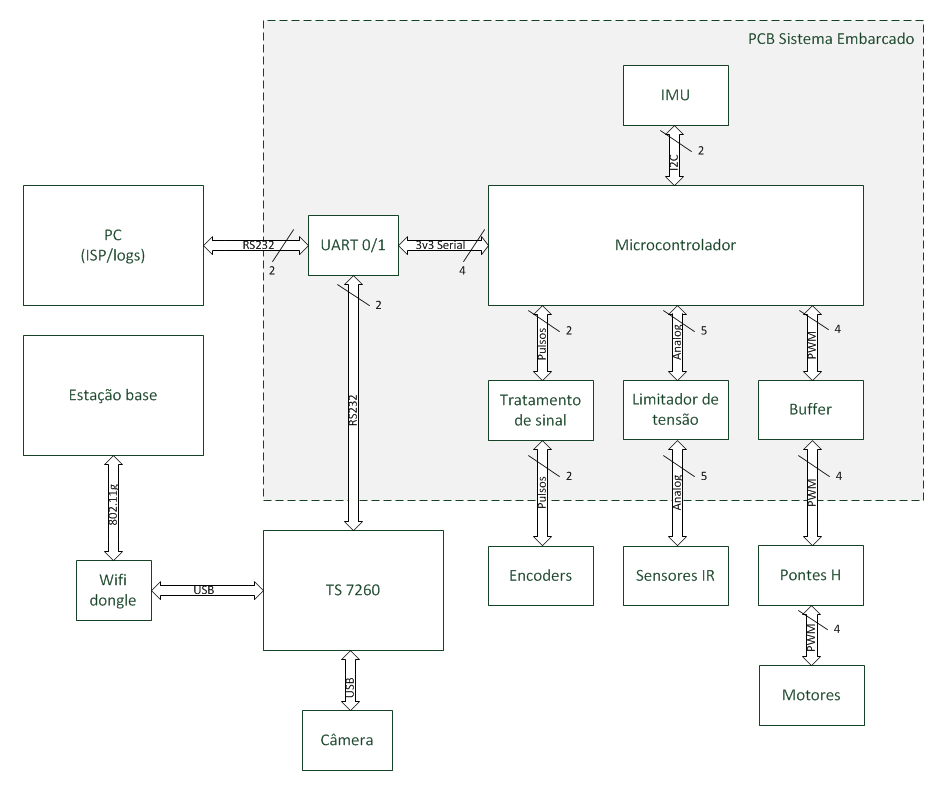
\includegraphics[width=\textwidth]{./figuras/diagrama_blocos_hardware.png}
  \caption{Diagrama de blocos do hardware}
  \label{fig:diagrama_blocos_hardware}
\end{figure}


\begin{enumerate}[topsep=0pt, partopsep=0pt, itemsep=0pt]
    \item Microcontrolador: Este bloco fará a leitura dos sensores: encoders, infra-vermelhos, acelerômetro e giroscópios. Além disso possui a implementação do protocolo de comunicação para interação com o linux embarcado da placa TS-7260.
    \item UART 0/1: Responsável por ajustar os níveis de tensão para comunicação serial no padrão RS-232 com a placa TS-7260.
    \item Buffer: Responsável por fornecer corrente e elevar os níveis de tensão de saída do microcontrolador de 3,3V para 5,0V. Esse buffer é conectado às pontes H já existentes no robô.
    \item IMU: possui o acelerômetro e o giroscópio e se comunicará com o microcontrolador por meio do protocolo I2C.
    \item Limitador de tensão: Necessário pois os sinais de saída dos sensores de infravermelho que já existem no robô não estão limitados em 5V, podendo a saída ultrapassar 5,0V e danificar o microcontrolador. 
    \item Tratamento de sinal: Composto por um filtro RC passa baixas e um schmitt trigger para remover qualquer falha que possa ocorrer na geração dos pulsos no encoder. A frequência de corte do filtro pode ser obtida pela velocidade máxima que o robô pode atingir, que foi suposta em 1 m/s (como apresentado nos requisitos de hardware).
\end{enumerate}

\section{Diagrama elétrico/eletrônico}

\begin{figure}[htpb!]
  \centering
  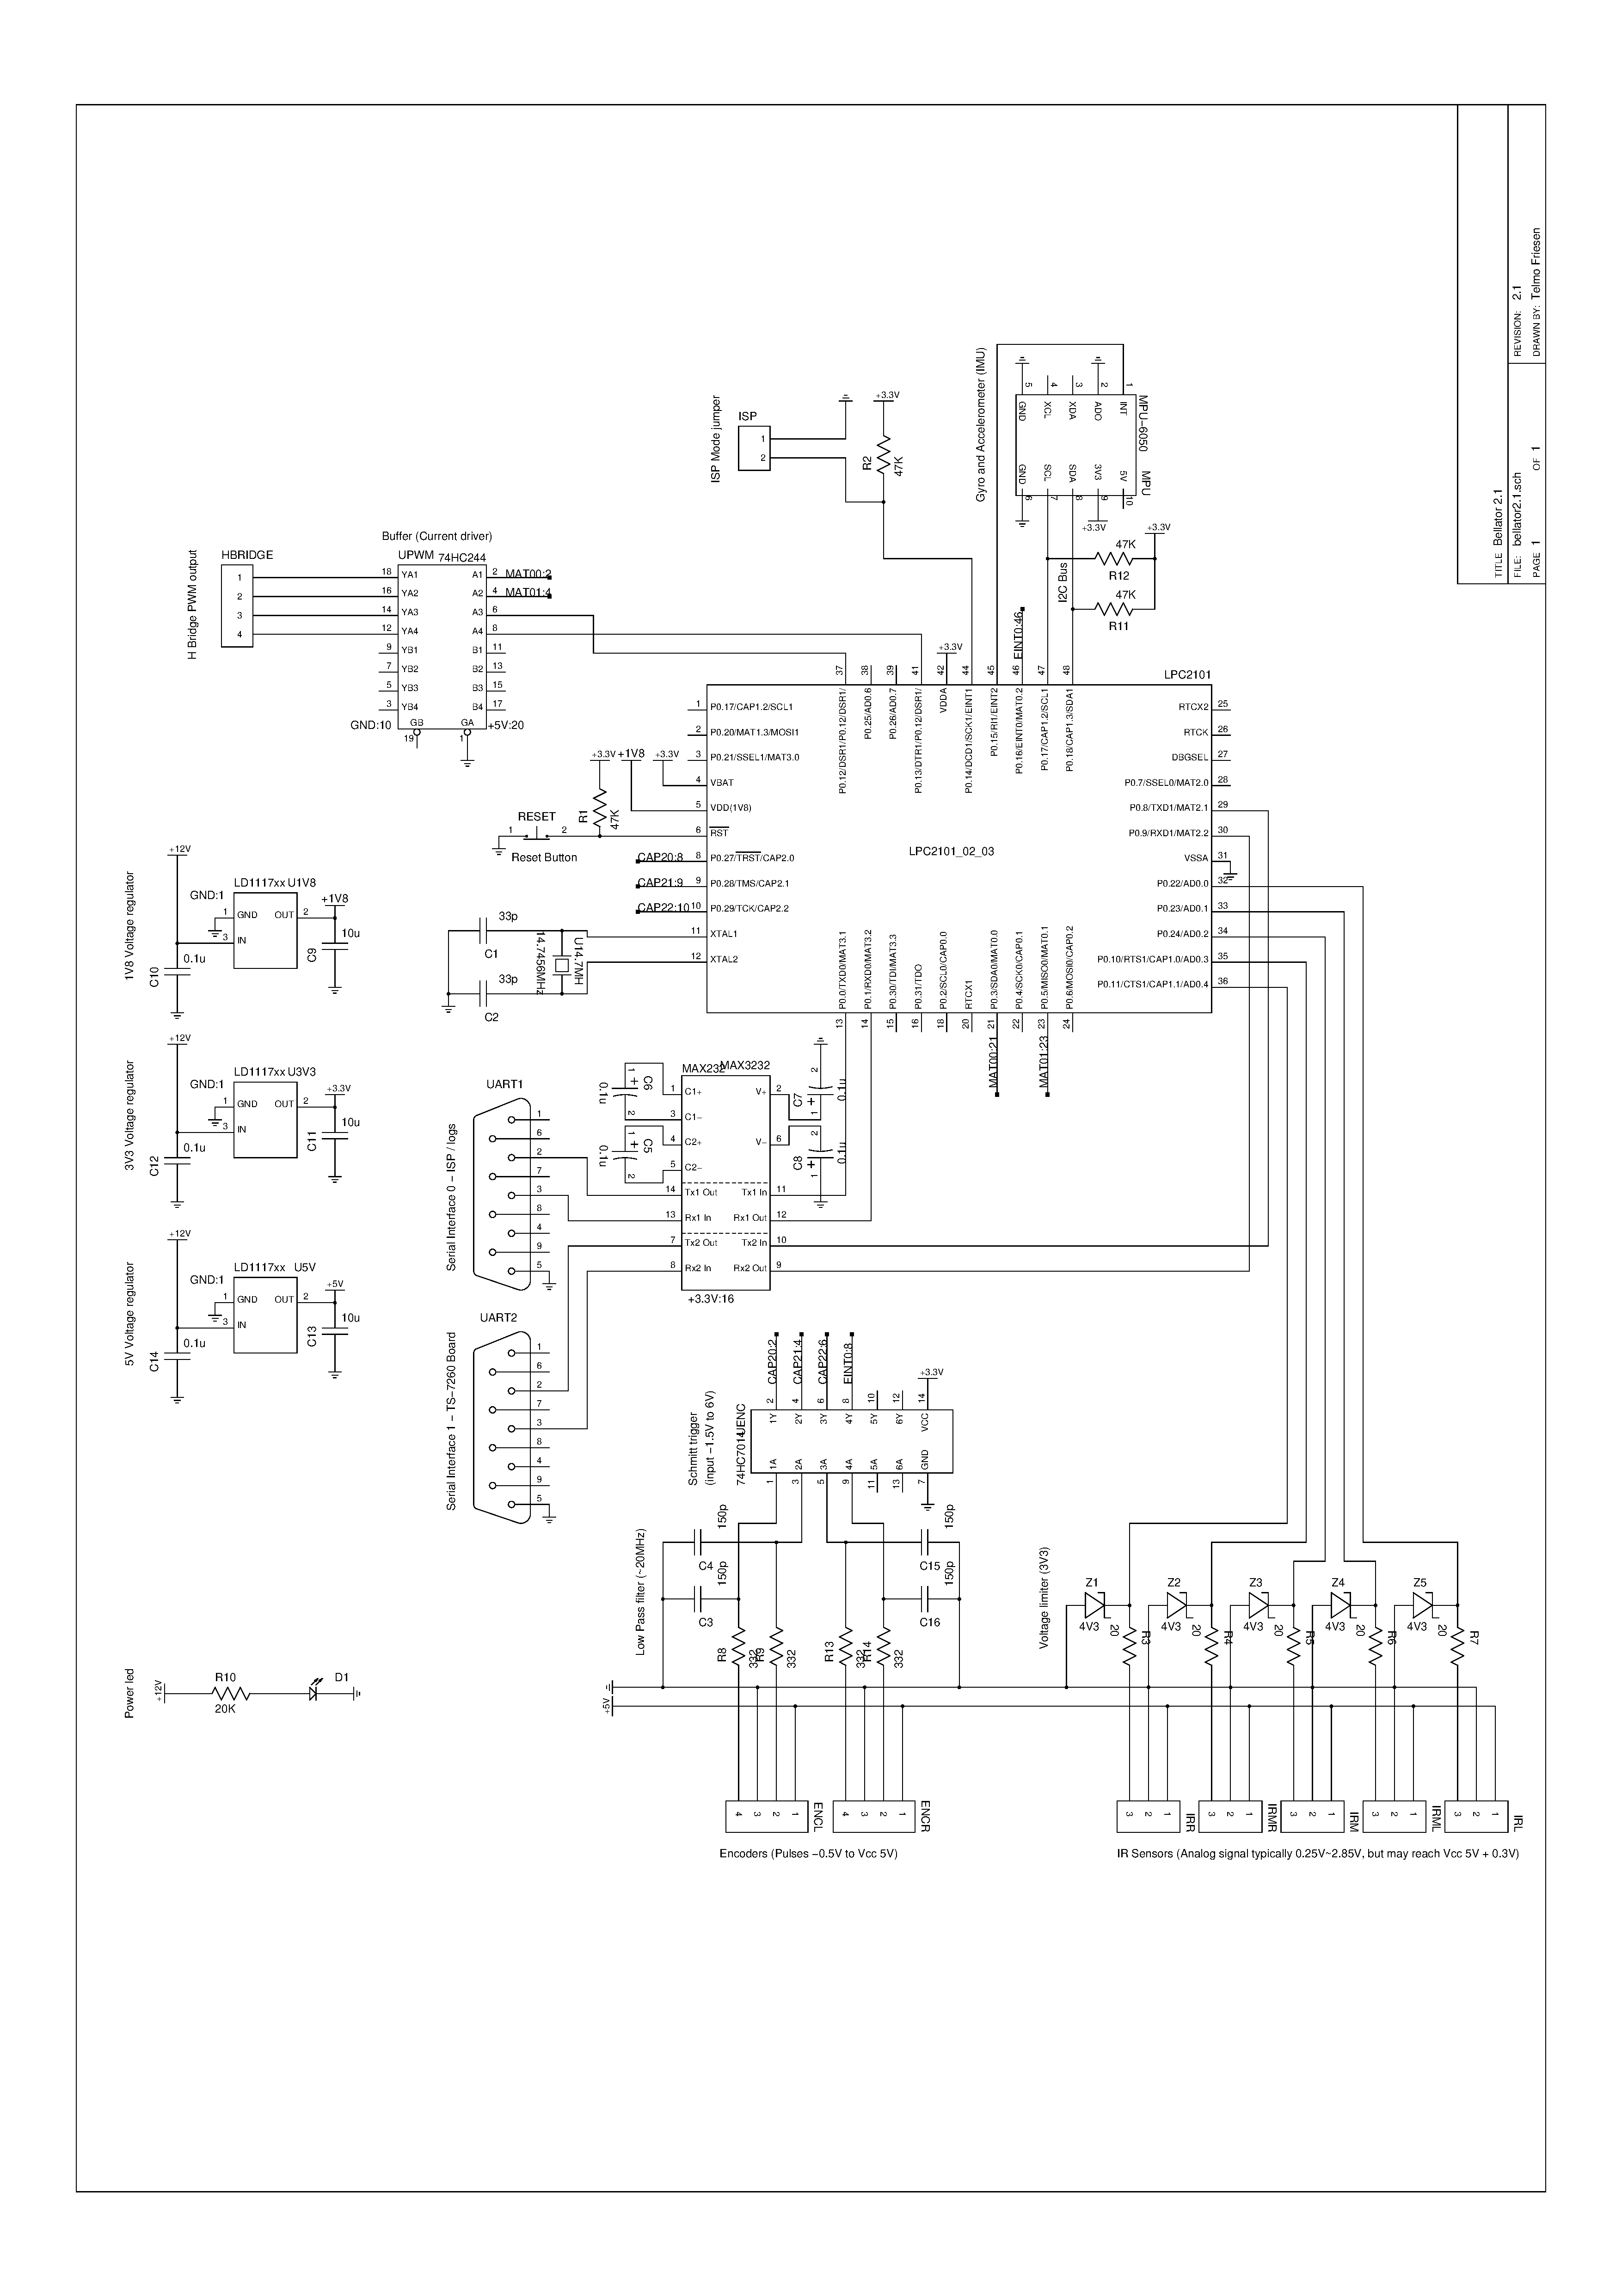
\includegraphics[width=0.9\textwidth, keepaspectratio]{./figuras/hardware2_1.pdf}
  \caption{Diagrama elétrico/eletrônico.}
  \label{fig:diagrama_eletrico_eletronico}
\end{figure}



